\documentclass[journal]{IEEEtran}

\usepackage[style=ieee]{biblatex} 
\usepackage{amsmath}
\usepackage{url}
\usepackage{graphicx}
\usepackage{float}

\usepackage{blindtext, subfig}
\usepackage{dblfloatfix}

% \usepackage[caption=false]{subfig}
\usepackage{todonotes}

\bibliography{ParticleSizeDistribution.bib}

\begin{document}

\title{Investigating Cross-Sectional Size Distribution of Randomly Distributed
       3D Spheres} 

\author{Sai Pandian, ID:\@ 29899923}%
        
% The report headers
\markboth{PHYS6017 Computer Techniques in Physics Report 2, May 2020}
{Shell \MakeLowercase{\textit{et al.}}: Bare Demo of IEEEtran.cls for IEEE Journals}

\maketitle

\begin{abstract}
  In this paper we present a 3-dimensional numerical simulation demonstrating
  that it is possible to reproduce the known planar cross-section distributions
  for Wicksell's Corpuscle Problem, thereby recovering 3D particle size
  distributions from 2D cross-sections. We investigate the effects of different
  particle sizes on the experimental data, and show this method is accurate for
  2 different starting 3D size distributions. We also present our findings on
  how sensitive this method is to experimental data and discuss its efficacy in
  a real world application such as identifying a material using a planar
  cross-section image from a microscope.
\end{abstract}

\section{Introduction}

\IEEEPARstart{I}{n} the world of Material Science and Crystallography, it is
often the case that a material is identified and classified using the
distribution of its constituent particle sizes. However, direct observation of
the particles so as to construct a distribution is often impossible. Using a
modern microscope or laser imaging techniques, it is possible to observe
particles in a cross-section of material. But the observed radii of particles in
this cross-section do not necessarily correspond directly to the radii of the
particles in the material, since the plane of the cross-section is not
necessarily oriented such that the observed particles lie exactly on the
plane. Thus, it becomes difficult to relate the observed distribution of
particle sizes in the plane to the real distribution of particle sizes in the
material.

Mathematically, determining the distribution of spherical particles from planar
sections is a well known problem called Wicksell's Corpuscle Problem
\cite{DWicksell}, named after S. D. Wicksell, who solved the problem in 1925. With
this solution, it is possible to determine the original distribution of
spherical particles. Thus, it is possible to determmine the distribution of
particle sizes in a solid from its observed cross-section, allowing us to
identify and classify materials better \cite{Cuzzi2016}.

In this paper we aim to show that it is possible to reproduce theoretical
results on cross-sectional distributions using numerical simulation, and it is
thus possible to solve Wicksell's Corpuscle Problem in this manner.


\section{Method}

Consider many spheres of different radii distributed randomly in space. For the
purposes of the numerical simulation, we will consider a cube of length 20. The
spheres were not allowed to overlap, which we ensured by placing the spheres such
that if one sphere has vector position $\overrightarrow{\textbf{a}}$ and radius
$r_{1}$ and the other has vector position $\overrightarrow{\textbf{b}}$ and
radius $r_{2}$, the spheres must have positions such that:
\begin{equation*}
|\overrightarrow{\textbf{a}} - \overrightarrow{\textbf{b}}| > (r_{1} + r_{2})
\end{equation*}
Random coordinates for a sphere are drawn from a uniform distribution and
checked against every existing sphere until a set of coordinates is drawn that
ensures no overlap, at which point the sphere is placed in space and the process
is repeated until all the necessary spheres have been placed.

\begin{figure}%[H]%[!ht]
\begin{center}
\includegraphics[width=0.45\textwidth]{./../Figures/box3d.pdf}
\caption{$750$ spheres of radius 0.7 distributed randomly in a cube of length 20,
  such that no sphere is touching or overlapping another sphere. A randomly
  oriented plane passes through the box and ``cuts'' through the
  spheres.}\label{fig:3dplot_plane}
\end{center}
\end{figure}

We then placed a plane into the cube, with a random orientation. The plane will
``cut'' through many of the spheres in the cube. This is shown in
Figure~\ref{fig:3dplot_plane}. Here we see $750$ spheres, each with radius 0.7
distributed randomly in a cube of length 20. The plane is shown in blue, and can
be seen intersecting many of the spheres in the cube.

In order to obtain the planar cross-section, we employed the spherical cap
method \cite{Sykes1922}. If we consider a sphere with centre
$\overrightarrow{\textbf{c}_0} = (x_0, y_0, z_0)$ and radius $R$, and a plane
with equation $Ax + By + Cz = D$ such that $\overrightarrow{\textbf{n}} = (A, B,
C)$ is the normal vector to the plane, then the distance from the centre of the
circle to the closest point on the plane $p_0$ is given by $\rho$:
\begin{equation*}
\rho = \frac{(\overrightarrow{\textbf{c}_0} - \overrightarrow{\textbf{p}_0}) \cdot{}
  \overrightarrow{\textbf{n}}}{|\overrightarrow{\textbf{n}}|} = \frac{Ax_0 +
  By_0 + Cz_0 - D}{\sqrt{A^2 + B^2 + C^2}}
\end{equation*}
If $|\rho| < R$, then there is an intersection of the plane and the sphere. The
radius of the circle $r$ in the planar cross-section is given by:
\begin{equation*}
r = \sqrt{R^2 - \rho^2}
\end{equation*}
And we then binned this radius to produce a histogram of the distribution of
planar circle radii. It is also possible to recover the centre
$\overrightarrow{\textbf{c}}$ of the circle visible on the plane using:
\begin{equation*}
\overrightarrow{\textbf{c}} = \overrightarrow{\textbf{c}_0} +
\rho\frac{\overrightarrow{\textbf{n}}}{|\overrightarrow{\textbf{c}}|} = (x_0,
y_0, z_0) + \rho\frac{(A, B, C)}{\sqrt{A^2 + B^2 + C^2}}
\end{equation*}

\begin{figure}%[H]%[!ht]
\begin{center}
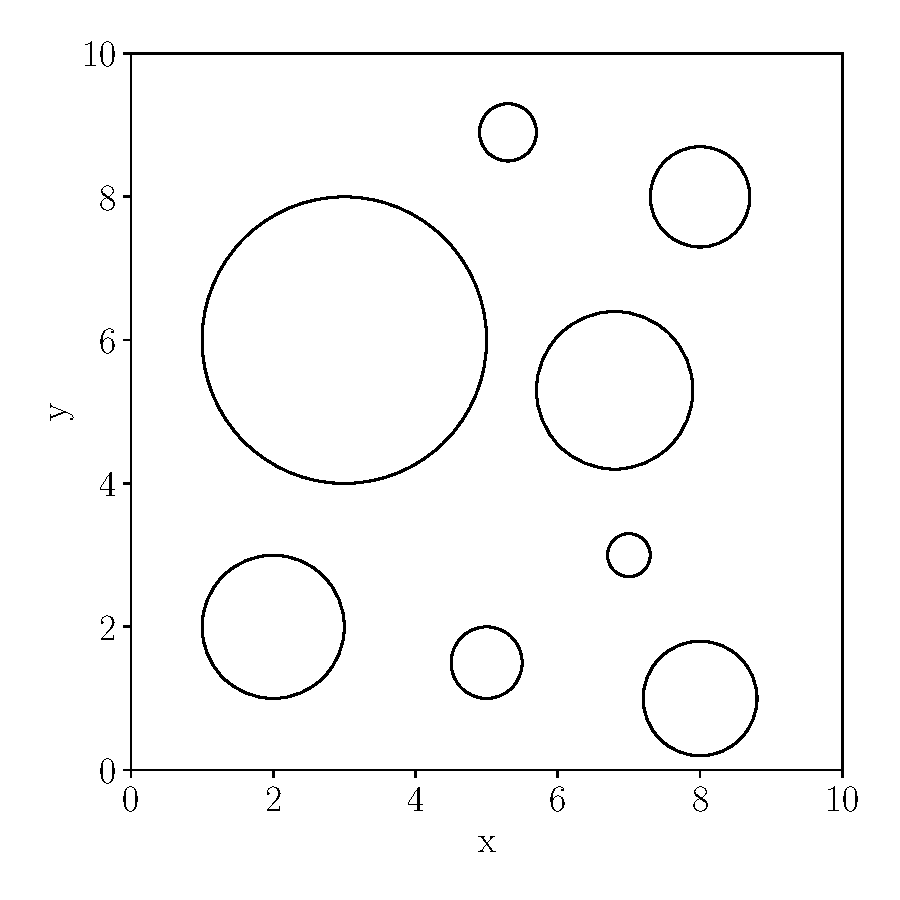
\includegraphics[width=0.45\textwidth]{./../Figures/circles.pdf}
\caption{Planar cross-section constructed using mock data. Spheres cut by the
  plane appear as circles on the plane, with radius dependent on the relative
  position of the spheres to the plane. This distribution of circles can be
  modelled.}\label{fig:circles}
\end{center}
\end{figure}

Figure~\ref{fig:circles} presents a planar cross-section generated using this
method and mock data. As we see, there are a range of circular radii observed
since even though the spheres all had the same radius, they were at different
distances from the plane, and were thus cut at different points. The many
observed circular radii are binned to produce a distribution.

If $f(R)dR$ is the number of spheres per unit volume with radii in interval $[R,
R + dR]$, then we can define a distribution $\phi(x)dx$ which represents the
number of circles per unit area on the plane with radii in interval $[x,
x+dx]$ \cite{Kiderlen2011}. This distribution is given by:
\begin{equation}
\phi(x) = \int_{x}^{\infty}\frac{xf(R)}{\sqrt{R^2 - x^2}}
\label{eq:phi_OG}
\end{equation}
We can compute this integral to obtain a theoretical planar distribution for
different starting spherical radius distributions.

We first considered the case in which all the spheres had the same radius
$R_0$. In this case, the spherical radius distribution is simply a Dirac delta
function centred on the radius $R_0$.

If we compute the integral in Equation~\ref{eq:phi_OG}, replacing $f(R)$ with
$\delta(R-R_0)$ we find:
\begin{equation}
\phi(x) = \int_{x}^{\infty}\frac{x\delta(R-R_0)}{\sqrt{R^2 - x^2}} =
\frac{xH(R_0-x)}{\sqrt{R_0^2-x^2}}
\label{eq:phi_constant}
\end{equation}
where $H(R_0 - x)$ is the heaviside function, which ``turns on'' the
distribution only for $x < R0$ as it is not possible to have a circular radius
$x$ larger than the spherical radius. So we aim to see our experimental data
reproduce this distribution. We also investigated how changing the
value of $R_0$ affects the experimental distribution.

We next considered the case in which each sphere has a radius $R$ uniformly
distributed in a range $R_1 < R < R_2$. In this case, we modify $f(R)$ in
Equation~\ref{eq:phi_OG} to be:
\begin{equation*}
  f(R) =
  \begin{cases}
    1,& \text{if } R_1 < R < R_2\\
    0,& \text{} Otherwise
  \end{cases}
\end{equation*}
In this case the integral in Equation~\ref{eq:phi_OG} does not need to be
computed with the limits shown, but instead with limits between $R_1$ and $R_2$
since $f(R)$ is 0 otherwise:

\begin{equation}
\begin{split}
  \phi(x) & = \int_{R_1}^{R_2}\frac{xf(R)}{\sqrt{R^2 - x^2}} \\
  = x\ln\left(\sqrt{R_2^2 - x^2}+R_2\right) & - x\ln\left(\sqrt{R_1^2 - x^2}+R_1\right)
\end{split}
\end{equation}
Since this distribution produces complex numbers for $ x < R_1$, we only
consider the real part of this distribution, which appears to produce a peak at
$x = R_1$.

\section{Results and Discussion}

We found that for both the case of the spheres of constant radius, and the case
of the spheres of varying radius, the experimental data reproduced a
distribution in the same shape as the theoretical distribution.

We first investigated the case where we placed $750$ spheres of radius $0.1$
each in a cube of length $20$. In this case we found that a plane in a random
orientation intersects very few spheres, since the spheres are very small. The
planar distribution is presented in Figure~\ref{fig:size1}.

\begin{figure}%[H]%[!ht]
\begin{center}
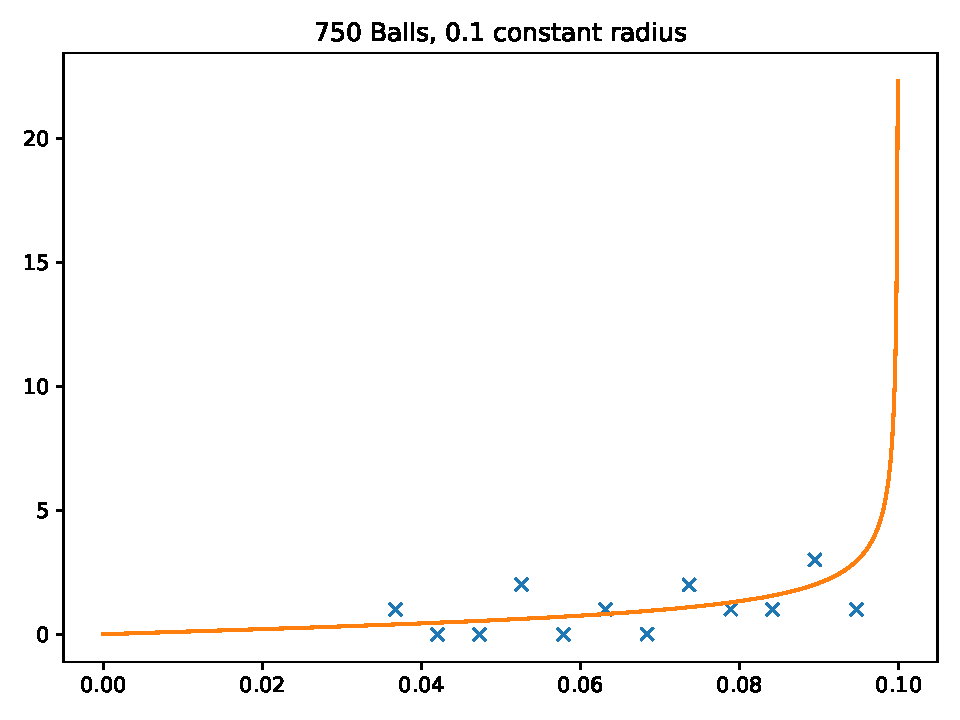
\includegraphics[width=0.45\textwidth]{./../Figures/750_01.pdf}
\caption{Distribution of circle radii on plane for $750$ spheres of radius $0.1$
  each. There are relatively few points since the spheres are small, so there is
  relatively small chance that they will be cut by the plane. So only a few
  circles are visible on the plane. The theoretical distribution is shown, with
  the experimental data matching this distribution, showing a slow increase in
  number or circles as radius increases.}\label{fig:size1}
\end{center}
\end{figure}

We observe relatively few experimental data points, as there were relatively few
intersections with the plane. This was likely because the spheres' radii were
very small compared to box length and there were relatively few spheres. While
the theoretical distribution shows a strong increase near $0.1$, this is not
evident from the experimental data. We also see that there is a lot of variance
between the points so the slow rise evident in the theoretical distribution is
not clear in the experimental data. It is thus necessary that we have more
spheres that intersect with the plane, in order to obtain a larger data-set.

We found that increasing the spheres' size or placing more spheres in the box,
or making the box length smaller, are all good methods of increasing the number
of intersections we observe, as they all increase the likelihood of intersection
by increasing the ratio of sphere occupied space to total box space. We thus
next used $750$ spheres of radius $0.3$ each. The planar cross-sectional
distribution found is presented in Figure~\ref{fig:size3}.

\begin{figure}%[H]%[!ht]
\begin{center}
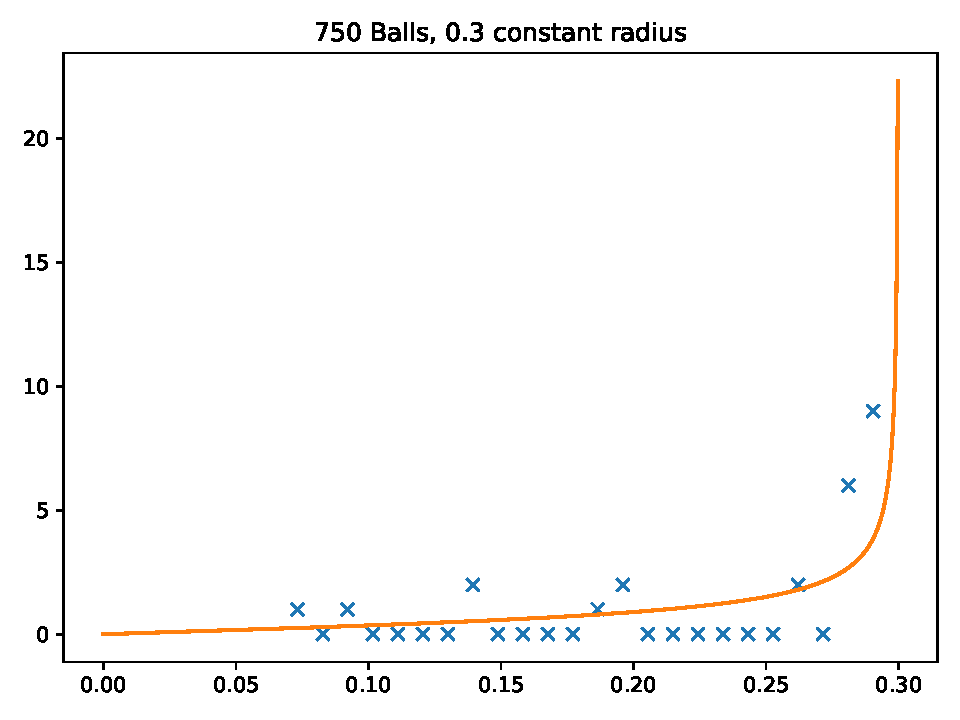
\includegraphics[width=0.45\textwidth]{./../Figures/750_03.pdf}
\caption{Distribution of circle radii on plane for $750$ spheres of radius $0.3$
  each. Compared to Figure~\ref{fig:size1}, there are many more experimental data
  points, since it is more likely that the plane will intersect these larger
  spheres. The experimental data more clearly resembles the theoretical
  distribution, showing a strong increase in number of circles as radius
  increases towards the maximum of 0.3.}\label{fig:size3}
\end{center}
\end{figure}

In Figure~\ref{fig:size3} we see that there are clearly more experimental data
points. This is because more spheres had intersections with the plane. Compared
to Figure~\ref{fig:1noise}, the slow rise in the theoretical distribution is
more closely followed by the experimental data. However, we still encounter
significant variance and fluctuation in lower radius bins, even though the
theoretical data is a smooth gradual increase. This is likely due to the
relatively few number of circles populating these bins, causing greater relative
difference between neighbouring bins. One method to solve this would be to use
fewer bins, which would have the effect of ``summing and averaging''
neighbouring bins so the experimental data has a smoother trend. However, this
would also reduce the number of data points so it was not implemented in our
investigation.

The sharp rise in the theoretical distribution close to the maximum radius is
also clear in the experimental data. It can be understood intuitively that we
expect to see more cross-sections with radius close to radius of the spheres
since there is a greater probability of intersection with the centre of a sphere
than any other point on the sphere.

\begin{figure}%[H]%[!ht]
\begin{center}
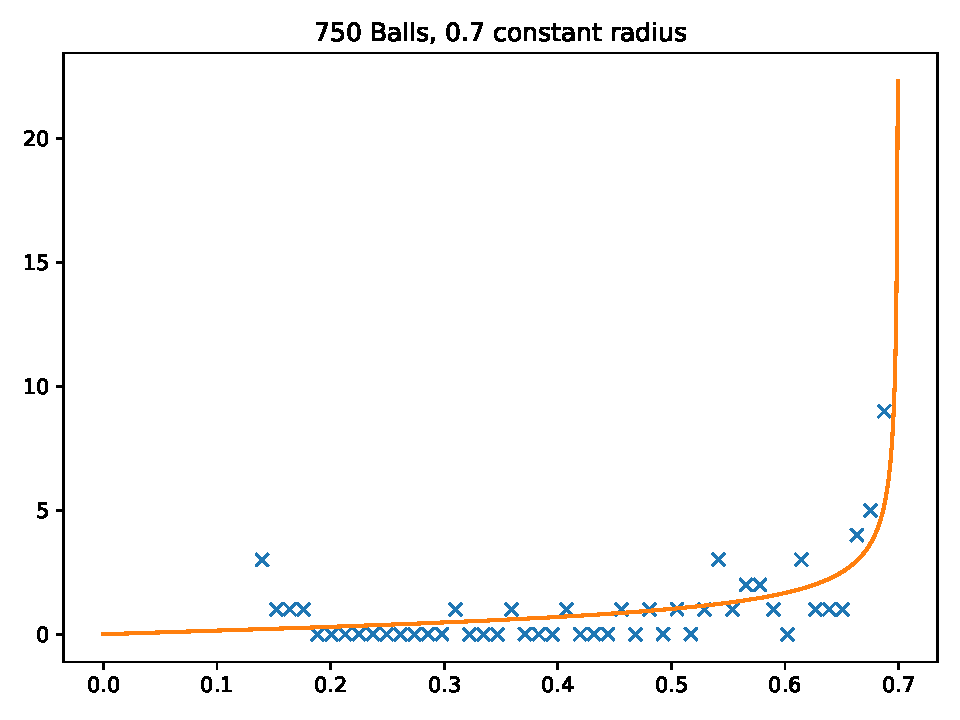
\includegraphics[width=0.45\textwidth]{./../Figures/750_07.pdf}
\caption{Distribution of circle radii on plane for $750$ spheres of radius $0.7$
  each. We do not observe much difference in how well the experimental data
  resembles the theoretical distribution between this figure and
  Figure~\ref{fig:size3}. With larger sized spheres, the simulation becomes harder
  to run as it is more difficult to randomly place spheres in a finite space
  without overlap.}\label{fig:size7}
\end{center}
\end{figure}

\begin{figure}[H]%[!ht]
\begin{center}
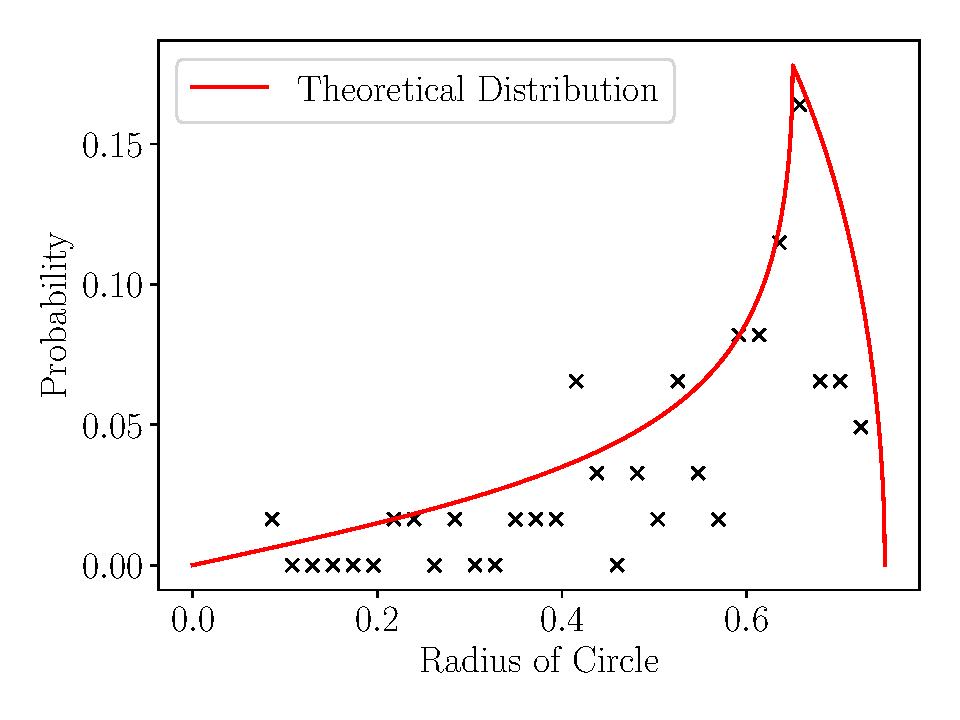
\includegraphics[width=0.45\textwidth]{./../Figures/750_07_random.pdf}
\caption{Distribution of circle radii on plane for $750$ spheres of radius $R$
  where $0.65 < R < 0.75$. The theoretical distribution is now different,
  although the experimental data still resembles this new distribution, showing
  a maximum around $R = 0.7$ and a sharp decrease after this. This is likely
  because there are more spheres with radii such that an overlap between $0$ and
  $0.7$ is possible, and relatively few spheres with radii such that a larger
  overlap is possible.}
\label{fig:random}
\end{center}
\end{figure}

\begin{figure*}[ht!]
  \centering
  \subfloat[Noise 2 orders of magnitude smaller than radius]
  {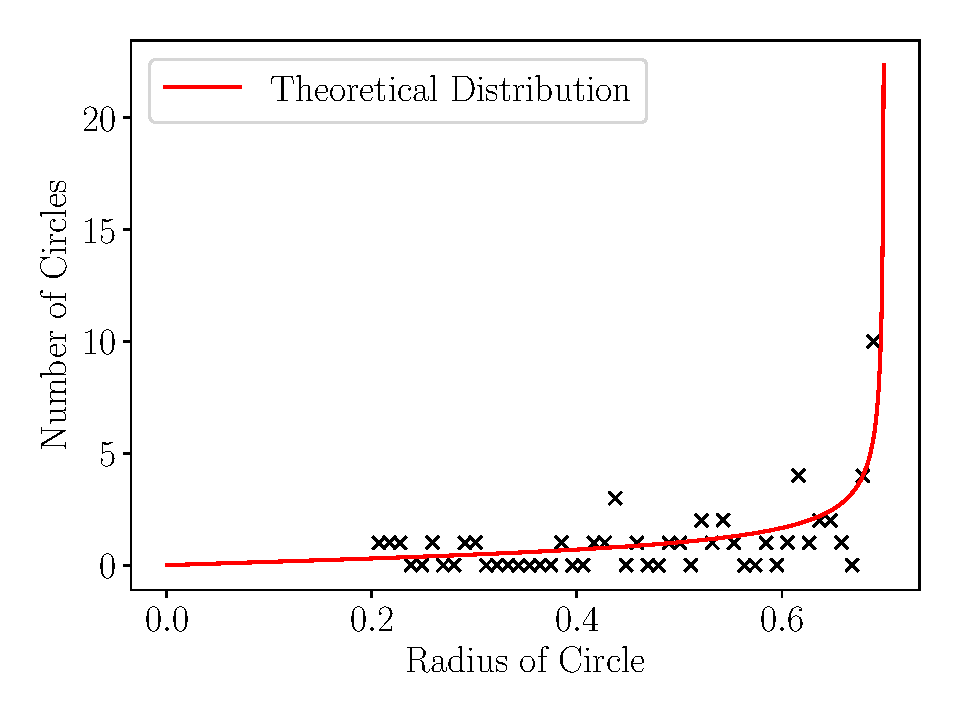
\includegraphics[width=0.45\textwidth]{./../Figures/750_07_Noise_100.pdf}
  \label{fig:2noise}}
  \centering
  \subfloat[Noise 1 order of magnitude smaller than radius]
  {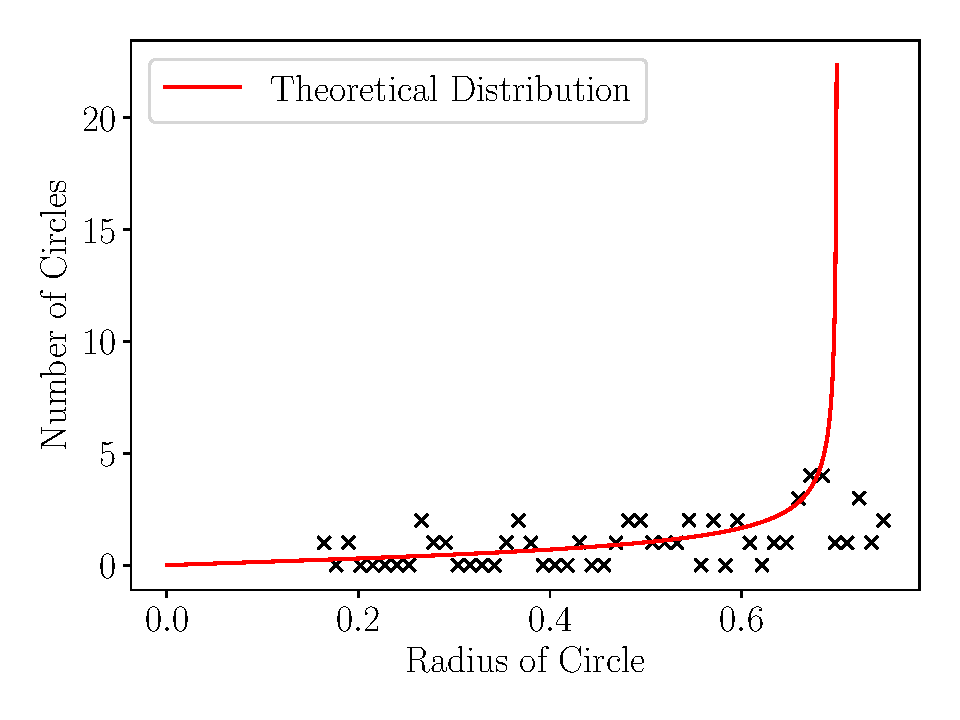
\includegraphics[width=0.45\textwidth]{./../Figures/750_07_Noise_10.pdf}
  \label{fig:1noise}}
  \caption{Distribution of circle radii on plane for $750$ spheres of radius $0.7$
    each. Each recorded radius has a random noise added to it in order to
    determine how sensitive the data is to experimental
    error. Figure~\ref{fig:2noise} shows the distribution for an added noise 2
    orders of magnitude smaller than the recorded radius, while
    Figure~\ref{fig:1noise} is the same for noise 1 order of magnitude smaller. As
    we can see, the experimental data very resembles the theoretical
    distribution when noise of 2 orders of magnitude smaller are added. But this
    is not true when noise of 1 order of magnitude smaller is added, implying
    the data is very sensitive to experimental data.}
  \label{fig:noiseplots}
\end{figure*}

Increasing the size of the spheres further to a radius of $0.7$, we might
initially expect the experimental data to resemble the theoretical distribution
even more closely, but this is not what we see. Figure~\ref{fig:size7} presents
the planar distribution for $750$ spheres of radius $0.7$ each.

In Figure~\ref{fig:size7}, we see a similar experimental distribution to that of
Figure~\ref{fig:size3}, as opposed to a distribution that more closely resembles
the theoretical distribution. While initially this may seem contrary to the
notion that increasing size of spheres would increase the number of
intersections and thus give a better distribution, this may simply be due to the
fact that increasing the size of the spheres beyond a certain radius does not
provide continually better results. We observe a similar number of intersections
as the case with spheres of radius $0.3$, and thus it is possible to conclude
that the best experimental distribution is found for a spherical size that
ensures a significant number of intersections. Though continually increasing
spherical size provides diminishing returns.


Indeed, we found that making the sphere sizes much larger made the placing of
the spheres in a finite space more difficult, and exponentially increased the
time complexity of the placing algorithm. This is because if the placed spheres
are too large, while it is initially easy to place spheres, as more are placed,
more coordinates must be randomly drawn before one if found for the next sphere
to be placed into. It is also possible that the algorithm never finds a possible
coordinate for later spheres. One possible solution to this may be to use a
better placing algorithm. Choosing a tight packing algorithm %\cite{Chen2001} would
maximise the number of spheres of a given radius that can be placed. However,
this would likely result in a less than random distribution of spheres if the
spheres are all of identical sizes. This would likely cause some systematic
error in the data, and so it was not investigated here. If we randomised the
sizes of the spheres as we do in the next part of the investigation, the problem
become significantly more complicated. Tight packing algorithms for irregular
shaped objects are very difficult to create and computationally expensive
\todo{cite}.

We next randomised the radius of each sphere to be in the range $0.65 < R <
0.75$. The experimental data for this simulation is presented in
Figure~\ref{fig:random}.

Figure~\ref{fig:random} presents the experimental data for 750 spheres with each
sphere having a radius $0.65 < R < 0.75$. As we can see, the theoretical
distribution has a very different shape to the case of constant sphere
radius. We see that the theoretical distribution has a sharp peak centred around
(but not precisely at) $0.65$, the lower limit of the uniform range the radii
were drawn from, and a sharp decrease after this point. This is likely due to
the higher number of spheres available in the box which could be intersected so
as to show a planar cross-section with radius $\approx 0.65$. In a range of
radii between $0.65 < R < 0.75$, all the spheres in the box can be intersected
so as to produce a circle of radius $0.65$, but there will be fewer spheres
which can be intersected to produce a circle of radius greater than this. So a
peak at this point and then a sharp decrease is expected.

The experimental data resembles the theoretical distribution, clearly showing a
peak and sharp decrease after. However, we also see that there is significant
variance between bins, and there is a large scatter around the theoretical
data. As explained for Figure~\ref{fig:size3}, it would be possible to reduce
this fluctuation by using fewer bins, at the cost of having fewer data
points. With a more powerful computer, or if the simulation is optimised and
written with a compiled language, there is also scope for significantly
increasing the size and number of spheres used, which would provide better
experimental data.

While there is significant fluctuation and scatter in all of the simulations
presented so far, the shapes of the distributions were mostly clear, and they
resembled the theoretical distribution. However, if the system is very sensitive
to experimental error, it may be difficult to identify distribution shapes, and
thus prevent us from properly identifying the starting distribution of spherical
radii. We therefore introduced some additional random error into the data. After
the radii of the circles on the plane are calculated, a small random number is
added to each radius. The random number is drawn from a uniform distribution in
the range $[\frac{-r}{n}, \frac{r}{n}]$, where r is the circle's radius and n is
the number of orders of magnitude we wish to choose the errors. We tested the
system with errors 2 orders of magnitude smaller than the radii and 1 order of
magnitude smaller than the radii. This is presented in
Figure~\ref{fig:noiseplots}. 


Figure~\ref{fig:2noise} presents the distribution for $750$ spheres or radius
$0.7$ each, with an added ``noise'' that is 2 orders of magnitude smaller than
each measured radius. We can see that the experimental data looks very similar
to the data presented in Figure~\ref{fig:size7}. The shape of the distribution
is also very clear and resembles the theoretical distribution.

Figure~\ref{fig:1noise} presents the same simulation but with an added noise
that is 1 order of magnitude smaller than each measured radius. Here we can see
that the experimental data is unrecognisable, and the shape of the distribution
is no longer clear. We thus conclude that the system is very sensitive to noise
greater than 2 orders of magnitude compared to the measured data.

However, it would be more prudent to use a Gaussian distribution to draw the
values of the noise. This is because it is likely that the many sources of error
possible in an experimental measurement of particle cross-sections in a material
will be convoluted together into a Gaussian distribution of errors due to the
central limit theorem \cite{Islam2018}. 

\section{Conclusions}
In this investigation we showed that it is possible to reproduce expected planar
distributions for the Corpuscle Problem with a 3-dimensional numerical
simulation of spheres distributed randomly in space, where a plane oriented
randomly intersects the spheres. We investigated how effective this method of
simulation is for different particle sizes, and showed that while initially
larger particles provide better data since they allow for more intersections,
continually increasing particle size becomes ineffective and computationally
expensive. 

We showed it was possible to reproduce the expected planar distributions for two
starting spherical radii distributions: a Dirac delta distribution, in which all
the spheres have the same radius, and a bounded uniform distribution, in which
all the spheres' radii are drawn randomly from a uniform distribution. Both
produce different shaped planar distributions but both provide data that
resembles the theoretical distributions.

We also investigated how sensitive this method is to experimental error. We
introduced some random noise into the system from a random uniform distribution
and demonstrated that the system is very sensitive to noise greater than two
orders of magnitude relative to measured data. Thus it is important for any
experimentalist making measurements of particle cross-sections in a material to
be very careful with error handling, as any error larger than 2 orders of
magnitude compared to measured data will result in great difficulty in
reproducing the spherical radii distributions.

We therefore showed in this investigation that it is possible to use the known
solutions to Wicksell's Corpuscle Problem to better identify and classify
materials by using planar measurements to gain information about 3D particle
distributions. 

\printbibliography{}
\end{document}
